\chapter{Suppressing the Fake Lepton Background}
For the simulated data used in this chapter, the \textsc{Sherpa} event generator was used for the signal $W+W+jj$ process, as well as the background processes: $Z+jets$, $ZZ$, $W+\gamma$, $W+jets$, and $WZ$. All diboson samples used the CT10 parton distribution function set \cite{CT10}. The single top and $t\bar{t}$ processes were generated by \textsc{PowHeg-Box}, and \textsc{Madgraph} was used for the $t\bar{t}+V$ process with showering algorithm handled by \textsc{Pythia}. $\uptau$-lepton decays were handled with the \textsc{Sherpa} parton showering algorithm. The output from each event generator was inputted into a GEANT4-based framework for detector simulation. The resulting MC samples were then post-processed, calibrated, and had some loose selection requirements applied to the physics objects. Unless otherwise stated, the object and event selections, as described in sections \ref{object_selection} and \ref{event_selection} respectively, were applied. The simulated data was normalised to an integrated luminosity of $28.0$fb$^{-1}$. The integrated luminosity was assumed was in line with the amount of run 2 data available for analysis when the simulated data was produced.
\section{Statistical Significance in Particle Physics}
In an experimental analysis, it is desirable to have as large an excess of signal events $s$ over expected background events $b$ as possible. This is commonly called the signal-to-background ratio $s/b$. In particle physics, Monte Carlo simulations are often used in order to determine an expected signal-to-background ratio, to more easily identify excesses in experimental data. Experimental analysis cuts are often optimised to maximise the signal-to-background ratio for this reason. However, in cases where the signal-to-background ratio is low but the number of total events is sufficiently large, signal excesses may still be identified and analysed regardless. Essentially being discrete counting experiments, statistical fluctuations in particle and nuclear physics experiments are Poissonian; i.e. $\sigma = \sqrt{N}$, where $N$ is the total number of event. The statistical significance is the number of standard deviations dividing a signal excess, thus since $N= s+b$, the significance in particle physics is given by:
$$ \frac{excess}{\sigma} = \frac{s}{\sqrt{s+b}}.$$ 
In practice, it is preferable to optimise based on the significance $s/\sqrt{s+b}$, rather than $s/b$, in instances where there is only a small signal excess relative to the total number of events.
\section{Optimising the $b$-jet Veto}
As mentioned in section \ref{intro_to_flb}, a veto on events found to contain a $b$-jet is used in the analysis of same-sign W-boson scattering events. This is used to suppress the non-prompt background, as the dominant contribution (see in table \ref{non-prompt_table}) comes from $t\bar{t}$ events where the top decays semi-leptonically, through emission of a $b$-quark. The means by which $b$-jets are identified in ATLAS is described in sub-section \ref{mva}. The multivariate $b$-tagger has four working points (see table \ref{b-tagger_working_points}), each with a corresponding efficiency. Implementing the $b$-tagger with the 85$\%$ efficiency means that the tagger will identify approximately 85$\%$ of all $b$-jets in a given event. The higher the efficiency of the $b$-tagger, the more jets will be tagged as being $b$-flavoured. Conversely, the purity (the percentage of tagged jets having $b$-flavour) decreases with efficiency. 
\begin{table}
	\centering{\begin{tabular}{|c|c|c|c|}
	\hline
	 & \multicolumn{3}{|c|}{non-prompt background} \\ \hline
	\textbf{$b$-jet veto} & $W$ + jets & $t\bar{t}$ & single top \\ \hline
	before & $79.54 \pm 38.19$ & $442.27 \pm 10.26$ & $37.43 \pm 2.12$ \\ \hline
	after & $77.15 \pm 38.17$ & $89.32 \pm 4.28$ & $12.71 \pm 1.22$ \\ \hline
	\end{tabular}}
	\caption{Number of events, across all channels, originating from each of the main contributors to the non-prompt background, before and after the $b$-jet veto is implemented. The multivariate $b$-tagger 70$\%$ efficiency working point was used. Note that $t\bar{t}$ events are are the dominant contributor. The cuts implemented before the veto are listed in chapter \ref{ssWW_analysis}. Errors displayed are purely statistical.}
	\label{non-prompt_table}
\end{table}

In order to determine the optimal multivariate $b$-tagger working point to use in the analysis of same-sign W-boson scattering, the significance at each working point is calculated and the working point at which the maximum significance occurs is designated the optimal working point. Recall that the other primary tools for reducing the fake lepton background, are the isolation selection requirements that are imposed on the lepton candidates. The multivariate $b$-tagger working point is optimised with all of the object selection criteria, including having the lepton candidates pass the \textit{Gradient} isolation selection requirement. It is also optimised for an alternate case, for when the lepton candidates are not required to pass any isolation selection requirements, as a control. This is not expected to perform as well as the \textit{Gradient} isolation selection requirement case as its lack makes it more likely that jet-faked leptons will pass the lepton candidate definitions. The working points are optimised individually for each analysis channel ($ee$, $e\mu +\mu e$, and $\mu\mu$) mentioned in section \ref{ssWW_intro}, as well as for the total across all channels. The ATLAS same-sign W-boson analysis is currently using the 85$\%$ efficiency working point.

Figure \ref{optimal_b-tagging_working_point_wGrad} and table \ref{b-tagging_working_point_wGrad_numbers} show the results of the optimisation study for the \textit{Gradient} isolation selection requirement case. Note that the maximum for the total over all channels occurs at the $70\%$ working point. For the $ee$, $e \mu + \mu e$, and $\mu\mu$ channels, the maximum significances occur at the $70\%$, $60\%$, and $70\%$ working points respectively. Also note that, aside from using the 0$\%$ efficiency (i.e. not having a $b$-jet veto), the currently used 85$\%$ efficiency working point performs the worst compared to all others. However, also note that the significances for all the non-zero efficiencies overlap within uncertainty. This is true per channel as well for the total.

On the other hand, figure \ref{optimal_b-tagging_working_point_noIso} and table \ref{b-tagging_working_point_noIso_numbers}, show the results of the alternate case for where the lepton candidates have no isolation selection requirements. Note that the maximum for the total over all channels occurs at the $70\%$ working point. For the $ee$, $e \mu + \mu e$, and $\mu\mu$ channels, the maximum significances occur at the $70\%$, $77\%$, and $70\%$ working points respectively. As with the first plot, the significances per channel as well as the total overlap within statistical uncertainty.

Comparing the two figures: note that the best approximation 3.38 of the maximum significance for the total across all channels, is achieved at the 70$\%$ efficiency, which is lower than that of the worst performing efficiency 0$\%$ working point for the first (requiring \textit{Gradient} isolation selection on lepton candidates) case, which has a best approximation to the significance of $3.46$. The values do overlap however, when the statistical uncertainty is taken into account. Like the first case, the 85$\%$ efficiency working point performs the worst when compared to the other non-zero efficiency working points.

While the two cases do not agree on the optimal working point for the $e\mu +\mu e$ channel, they are both in agreement that the $70\%$ multivariate working point performs best when considering the best approximations to the significance. These results considering the best approximations to the significance alone suggest moving from the currently used 85$\%$ efficiency working point to the 70$\%$ efficiency working point. This would increase the significance by approximately 5$\%$. The reason for this is that while the 85$\%$ efficiency working point tags more events containing a $b$-jet (and hence vetoes more background events), it also vetoes more signal events. This can be seen from the numbers in table \ref{b-tagging_working_point_wGrad_numbers}, where in the 85$\%$ efficiency, the background decreases by 12$\%$ compared to the 70$\%$ efficiency. However, the signal also decreases by 11$\%$, and due to the significance quantity $s/\sqrt{s+b}$ being more sensitive to decreases in signal events, this has the effect of resulting in an overall lower significance for the 85$\%$ efficiency working point when compared to the 70$\%$ working point. This study suggests then that the optimal $b$-tagger efficiency is the 70$\%$ working point. It should be stressed however, that this is a weak assertion given that, when the uncertainties are taken into account, the differences in the significances between each efficiency working point are not statistically significant, i.e. it could be a statistical fluctuation. Further studies, using larger sample sizes are necessary to determine whether to move to efficiency working point from 85$\%$ to 70$\%$ is warranted.

The studies also suggest that the \textit{Gradient} isolation selection has the effect of increasing the significance across all channels and efficiency working points. This was not, however, unexpected.
\begin{table}
	\resizebox{\textwidth}{!}{\centering{\begin{tabular}{|l|c|c|c|c|c|}
	\hline
	Working Point & $0\%$ & $60\%$ & $70\%$ & $77\%$ & $85\%$ \\ \hline \hline
	$ee$ bkg. & $30.83 \pm 4.02$ & $19.36 \pm 3.67$ & $18.26 \pm 3.64$ & $17.38 \pm 3.62$ & $16.30 \pm 3.59$ \\ \hline
	$e\mu + \mu e$ bkg. & $46.16 \pm 3.02$ & $29.72 \pm 2.49$ & $28.57 \pm 2.47$ & $26.61 \pm 2.38$ & $26.61 \pm 2.38$ \\ \hline
	$\mu\mu$ bkg. & $19.77 \pm 1.54$ & $16.20 \pm 1.48$ & $15.06 \pm 1.39$ & $14.32 \pm 1.36$ & $12.56 \pm 1.27$ \\ \hline
	total bkg. & $96.76 \pm 5.26$ & $67.07 \pm 4.70$ & $63.06 \pm 4.62$ & $60.27 \pm 4.59$ & $55.47 \pm 4.49$ \\ \hline
	$ee$ sig. & $5.82 \pm 0.13$ & $5.71 \pm 0.13$ & $5.59 \pm 0.12$ & $5.43 \pm 0.12$ & $4.99 \pm 0.12$ \\ \hline
	$e \mu + \mu e$ sig. & $20.71 \pm 0.24$ & $20.26 \pm 0.24$ & $ 19.86 \pm 0.23$ & $19.25 \pm 0.23$ & $17.67 \pm 0.22$ \\ \hline
	$\mu\mu$ sig. & $14.01 \pm 0.20$ & $ 13.74 \pm 0.19$ & $13.48 \pm 0.19$ & $13.08 \pm 0.19$ & $11.98 \pm 0.18$ \\ \hline
	total sig. & $40.54 \pm 0.34$ & $39.71 \pm 0.33$ & $38.93 \pm 0.32$ & $37.76 \pm 0.32$ & $34.64 \pm 0.31$ \\ \hline
	total $s/\sqrt{s+b}$ & $3.46 \pm 0.07$ & $3.843 \pm 0.09$ & $3.86 \pm 0.09$ & $3.81 \pm 0.09$ & $3.65 \pm 0.10$ \\ \hline
	\end{tabular}}}
\caption{Number of signal and background events by channel and multivariate $b$-tagger efficiency working point. The total significance is given in the bottom row for each efficiency working point. The lepton candidates must pass the \textit{Gradient} isolation selection requirement. Errors displayed are purely statistical}
\label{b-tagging_working_point_wGrad_numbers}
\end{table}
\begin{table}
	\resizebox{\textwidth}{!}{\centering{\begin{tabular}{|l|c|c|c|c|c|}
	\hline
	Working Point & $0\%$ & $60\%$ & $70\%$ & $77\%$ & $85\%$ \\ \hline \hline
	$ee$ bkg. & $41.62 \pm 4.32$ & $26.18 \pm 3.88$ & $24.45 \pm 3.85$ & $22.99 \pm 3.81$ & $21.26 \pm 3.78$ \\ \hline
	$e\mu + \mu e$ bkg. & $82.76 \pm 4.21$ & $55.16 \pm 3.50$ & $51.29 \pm 3.42$ & $47.64 \pm 3.32$ & $43.11 \pm 3.19$ \\ \hline
	$\mu\mu$ bkg. & $50.45 \pm 9.22$ & $39.17 \pm 9.11$ & $36.95 \pm 9.08$ & $35.26 \pm 9.06$ & $31.99 \pm 9.04$ \\ \hline
	total bkg. & $174.83 \pm 11.02$ & $120.51 \pm 10.50$ & $112.69 \pm 10.44$ & $105.89 \pm 10.37$ & $96.36 \pm 10.30$ \\ \hline
	$ee$ sig. & $6.22 \pm 0.13$ & $6.09 \pm 0.13$ & $5.96 \pm 0.13$ & $5.78 \pm 0.13$ & $5.32 \pm 0.12$ \\ \hline
	$e \mu + \mu e$ sig. & $22.41 \pm 0.25$ & $21.91 \pm 0.25$ & $ 21.46 \pm 0.24$ & $20.81 \pm 0.24$ & $19.08 \pm 0.23$ \\ \hline
	$\mu\mu$ sig. & $15.20 \pm 0.20$ & $14.91 \pm 0.20$ & $14.63 \pm 0.20$ & $14.19 \pm 0.20$ & $13.02 \pm 0.19$ \\ \hline
	total sig. & $43.83 \pm 0.35$ & $42.91 \pm 0.34$ & $42.05 \pm 0.34$ & $40.78 \pm 0.34$ & $37.42 \pm 0.32$ \\ \hline
	total $s/\sqrt{s+b}$ & $2.96 \pm 0.08$ & $3.36 \pm 0.11$ & $3.38 \pm 0.12$ & $3.37 \pm 0.12$ & $3.24 \pm 0.13$ \\ \hline
	\end{tabular}}}
\caption{Number of signal and background events by channel and multivariate $b$-tagger efficiency working point. The total significance is given in the bottom row for each efficiency working point. The lepton candidates are not required to pass any isolation selection criteria. Errors displayed are purely statistical.}
\label{b-tagging_working_point_noIso_numbers}
\end{table}
\begin{figure}
\centering{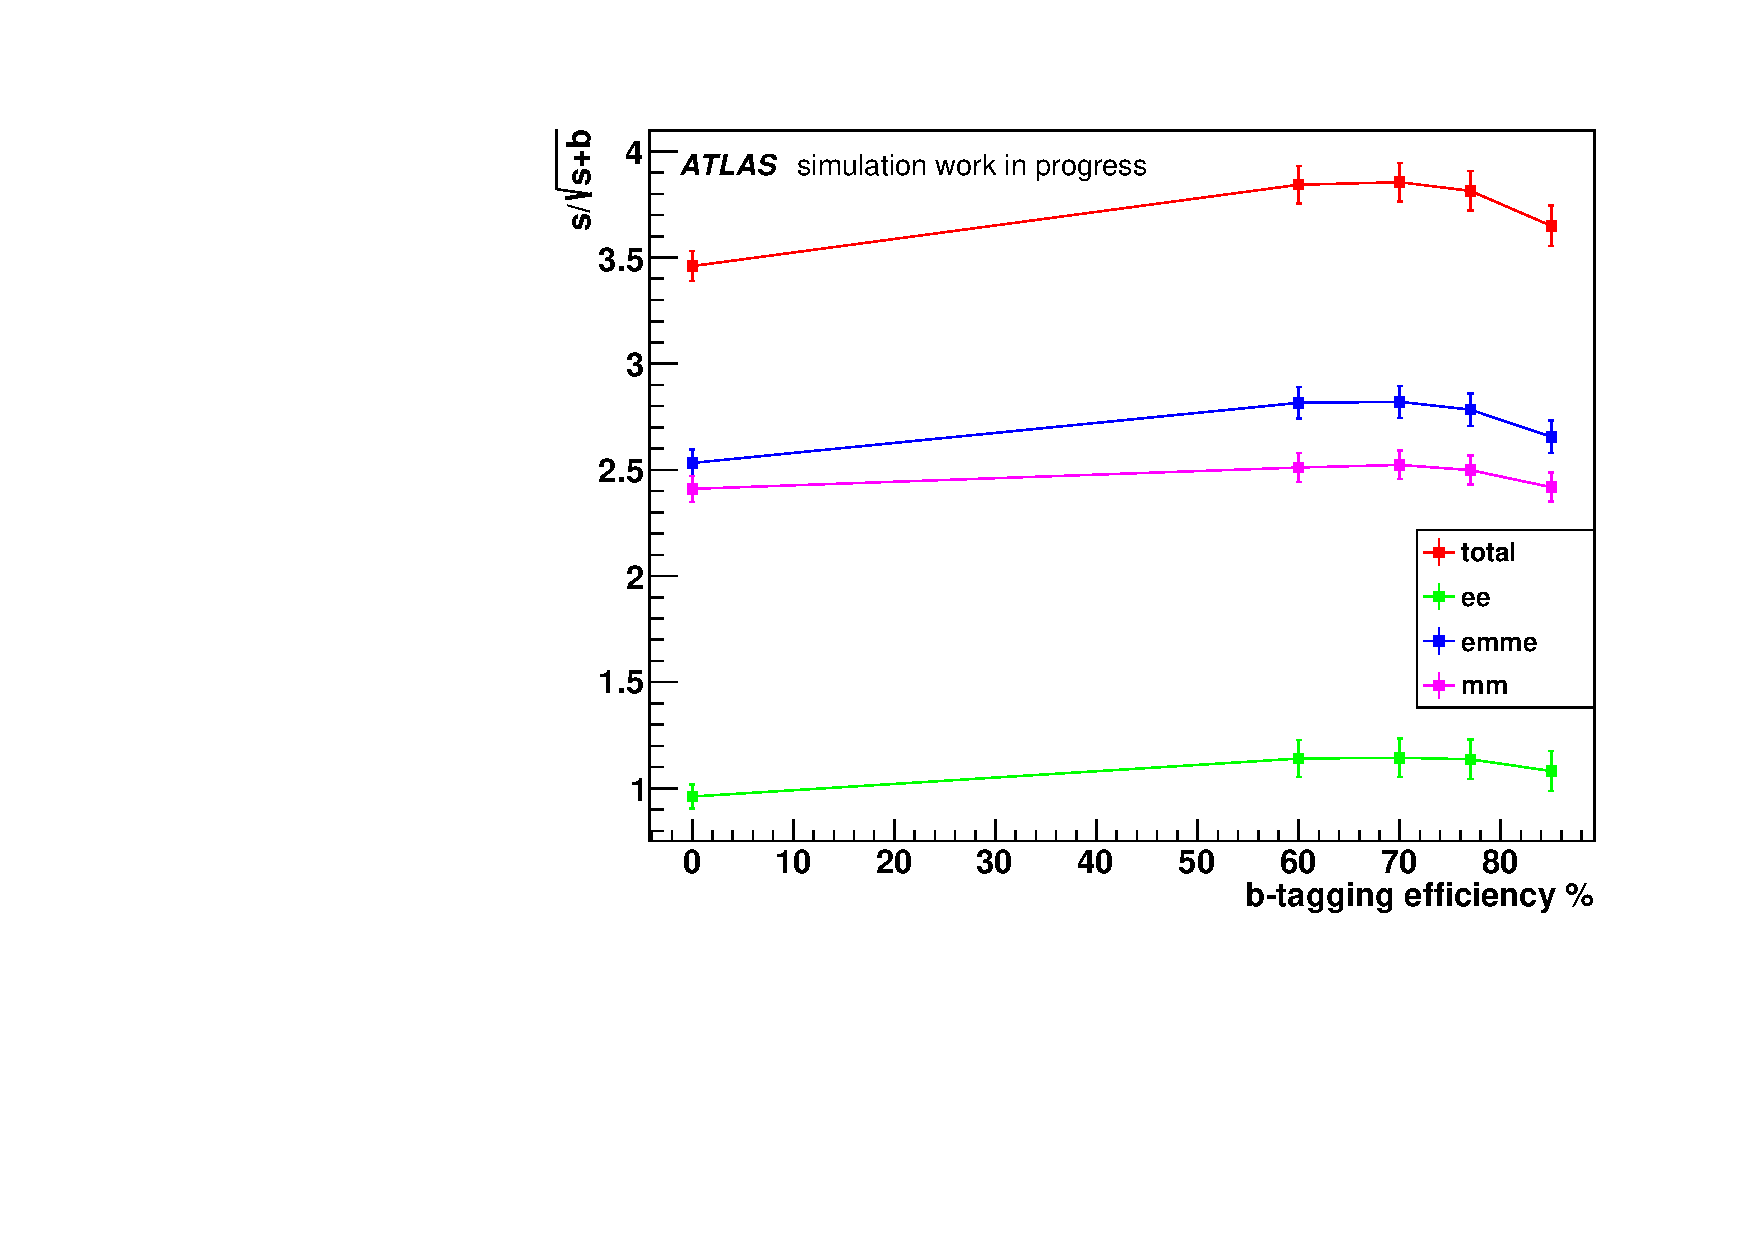
\includegraphics[width=1.\textwidth]{images/chapter7/Grad_stbr_btag_better.pdf}}
\caption{The significance at each multivariate $b$-tagger working point as well as the significance at $0\%$ (which corresponds to not using a $b$-jet veto at all). Lepton candidates were required to pass the \textit{Gradient} isolation requirement.}
\label{optimal_b-tagging_working_point_wGrad}
\end{figure}
\begin{figure}
\centering{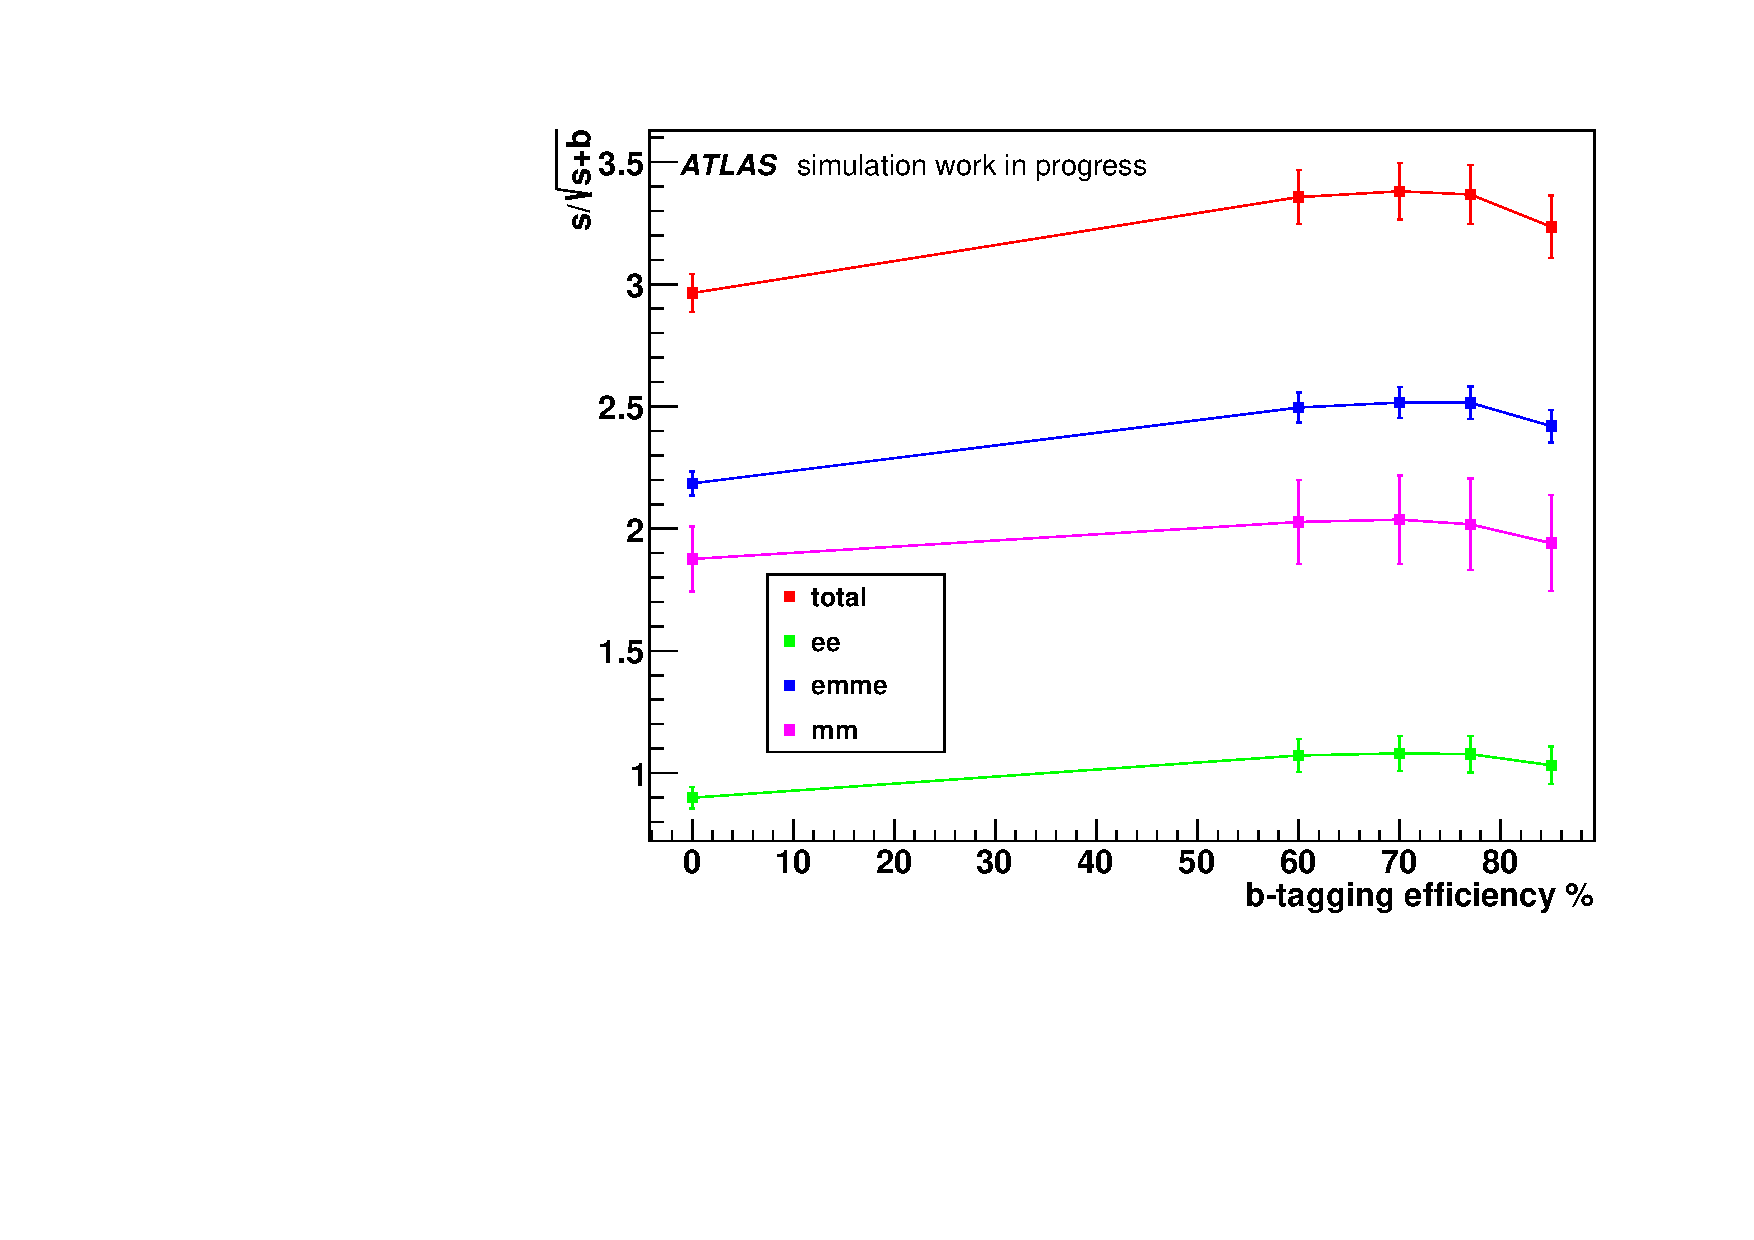
\includegraphics[width=1.\textwidth]{images/chapter7/noIso_stbr_btag_better.pdf}}
\caption{The significance at each multivariate $b$-tagger working point as well as the significance at $0\%$ (which corresponds to not using a $b$-jet veto at all). No isolation selection requirements were imposed on the lepton candidates.}
\label{optimal_b-tagging_working_point_noIso}
\end{figure}
\section{Optimising the Isolation Requirements for Lepton Candidates}
\subsection{The Cumulative Significance}
\label{description_of_cum_sig}
As stated in section \ref{intro_to_flb}, imposing an isolation requirement on the same-sign W-boson scattering lepton candidates is a technique for suppressing the \emph{fake lepton background}. The optimisation of the multivariate $b$-tagger was done by requiring candidate leptons to pass the \textit{Gradient} isolation selection working point (described in section \ref{iso_wps}). This section will be concerned with determining the optimal working point for the isolation selection; whether it be a fixed cut, a targeted efficiency such as \textit{Gradient}, or some composition of the two. Optimisation is based on the \emph{cumulative significance} quantity, defined as
$$
s_{cum}/\sqrt{s_{cum}+b_{cum}},
$$
where $s_{cum}$ is the sum of all signal events up to a given point being considered and similarly $b_{cum}$ is the sum of all background events up to that same point.

In order to determine how to use the cumulative significance to determine optimal analysis cuts, it is useful to plot it for a variety of artificial set-ups. However, first it is necessary to derive the uncertainty on the cumulative significance, in order to produce correct error bars necessary for comparison. For a function $f(x,y)$, the uncertainty is given by \cite{lyons}:
\begin{equation}
\sigma_{f}^{2} \approx \left| \frac{\partial f}{\partial x} \right| \sigma_{x}^{2} + \left| \frac{\partial f}{\partial y} \right| \sigma_{y}^{2}.
\end{equation}
Then if the cumulative significance is denoted $\alpha$, the uncertainty is:
\begin{equation}
\sigma_{\alpha}^{2} \approx \left| \frac{\partial \alpha}{\partial s_{cum}} \right| \sigma_{s_{cum}}^{2} + \left| \frac{\partial \alpha}{\partial b_{cum}} \right| \sigma_{b_{cum}}^{2}.
\end{equation}
Evaluating, gives:
\begin{equation}
\sigma_{\alpha}^{2} = \frac{s_{cum}+2b_{cum}}{2(s_{cum}+b_{cum})^{3/2}}\sigma_{s_{cum}}^{2} -\frac{s_{cum}}{2}\left( s_{cum} + b_{cum} \right)^{-3/2}\sigma_{b_{cum}}^{2},
\end{equation}
which is then used for the error bars subsequently.

Figures \ref{test_cum_sig} and \ref{test_cum_sig_rev} each display signal and background contributions for an arbitrary variable in a hypothetical experiment. In figure \ref{test_cum_sig}, the upper plots show two artificial set-ups where the signal contribution abruptly goes to zero at $x=6$, with the corresponding cumulative significance plotted below for each. In the upper right plot, the background contribution is constant at 25 across the entire $x$-range whereas the signal contribution is constant at 6 until the point $x=6$, after which it is zero. In the top left plot, the background contribution linearly increases whereas the signal contribution is constant at 6 until the point $x=6$ in the same way as the upper right plot. The cumulative significance of both the left and right set-ups peaks at the point where the signal goes to zero and then gradually decreases. This suggests placing an upper bound cut at $x = 6$ in order to maximise the cumulative significance.

Conversely, in figure \ref{test_cum_sig_rev}, the upper plots show two artificial set-ups where the signal contribution abruptly goes to 6 at $x=20$, with the corresponding cumulative significance plotted below for each. In the upper right plot, the background contribution is constant at 25 across the entire $x$-range whereas the signal contribution is constant at zero until the point $x=25$, after which it is 6. In the top left plot, the background contribution linearly decreases whereas the signal contribution is constant at zero until point $x=25$, in the same way as the upper right plot. The cumulative significance of both the left and right set-ups is zero until $x=25$, after which it grows rapidly. This suggests placing an lower bound cut at $x = 25$ in order to maximise the cumulative significance.

\begin{figure}\centering{
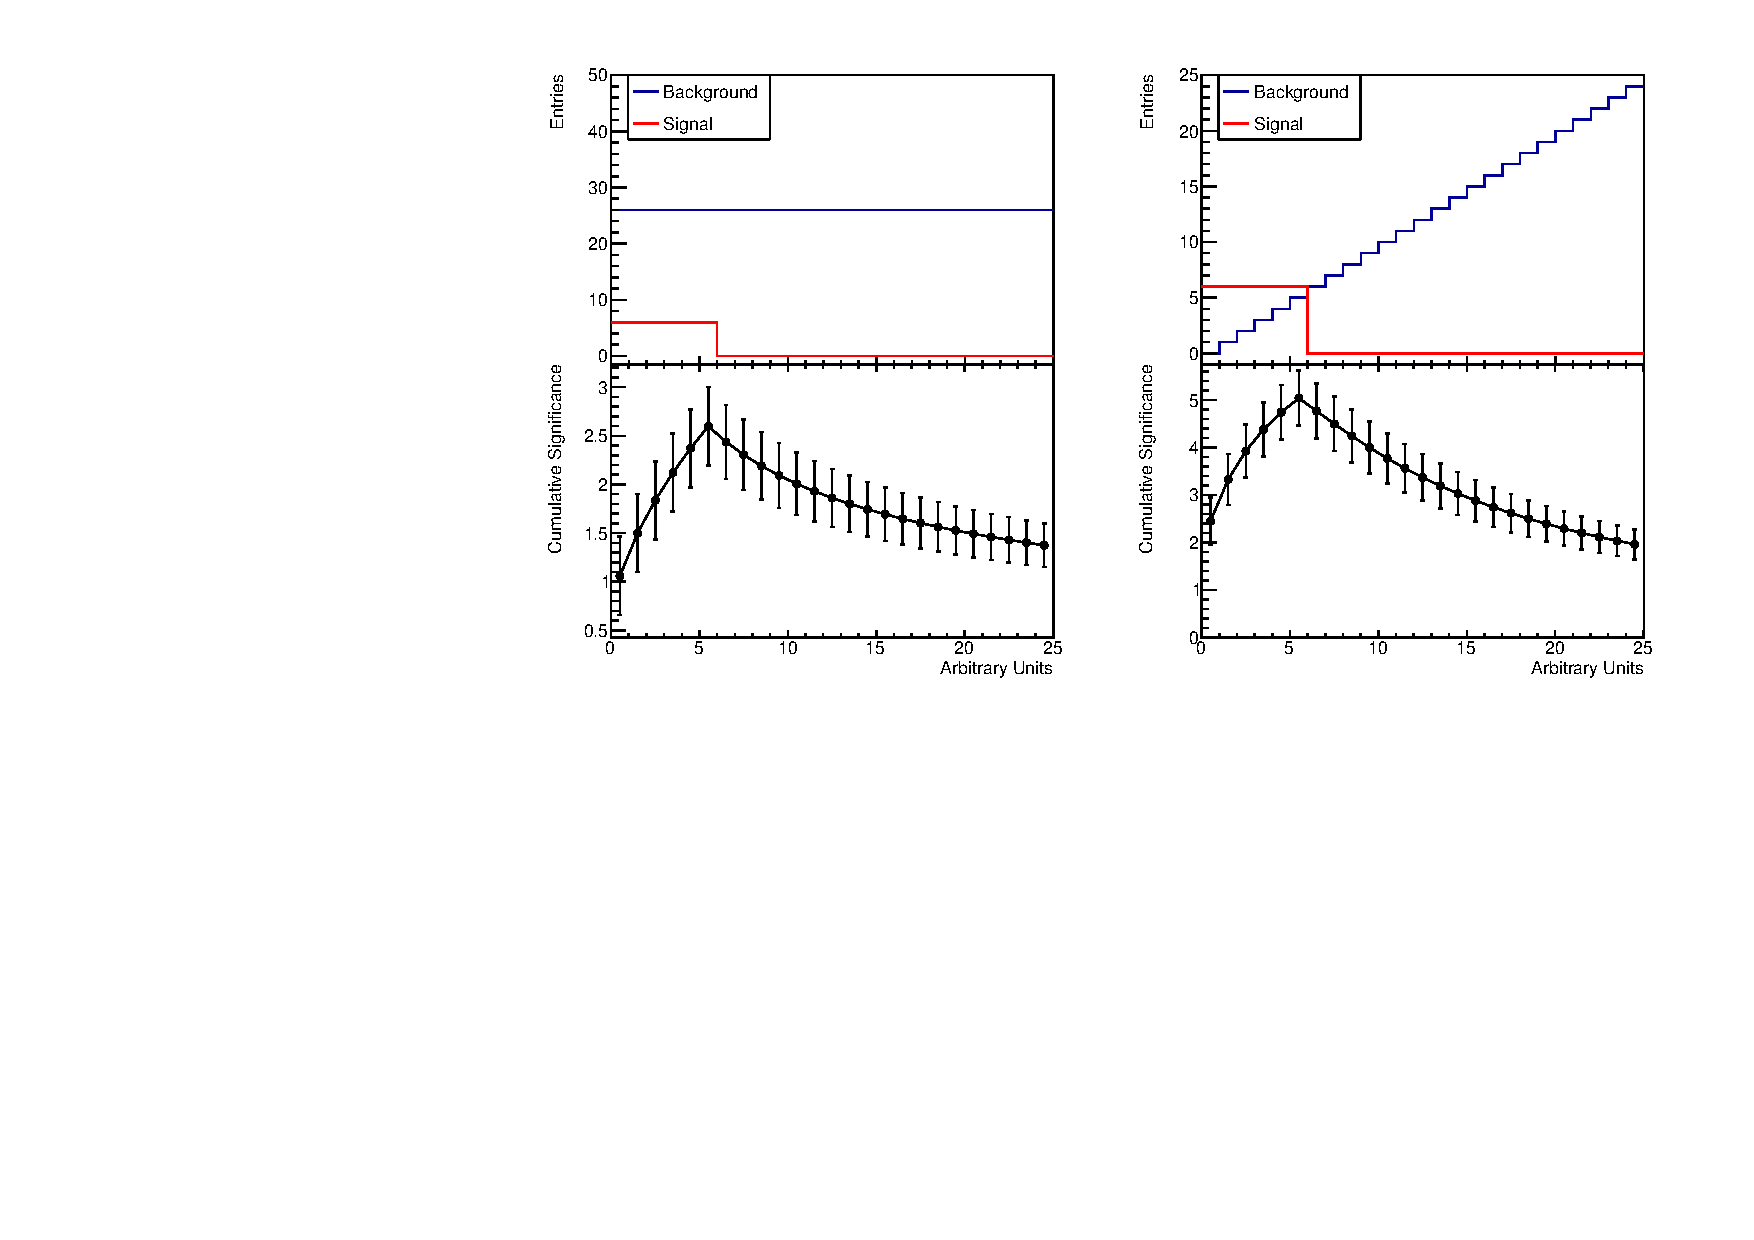
\includegraphics[width=1.\textwidth]{images/chapter7/test_cum_sig.pdf}
\caption{Two distinct artificial experimental setups, with the corresponding cumulative significances plotted below. Note the distinctive peak near $x=6$, indicating the optimal cut location.}
\label{test_cum_sig}
}\end{figure}
\begin{figure}\centering{
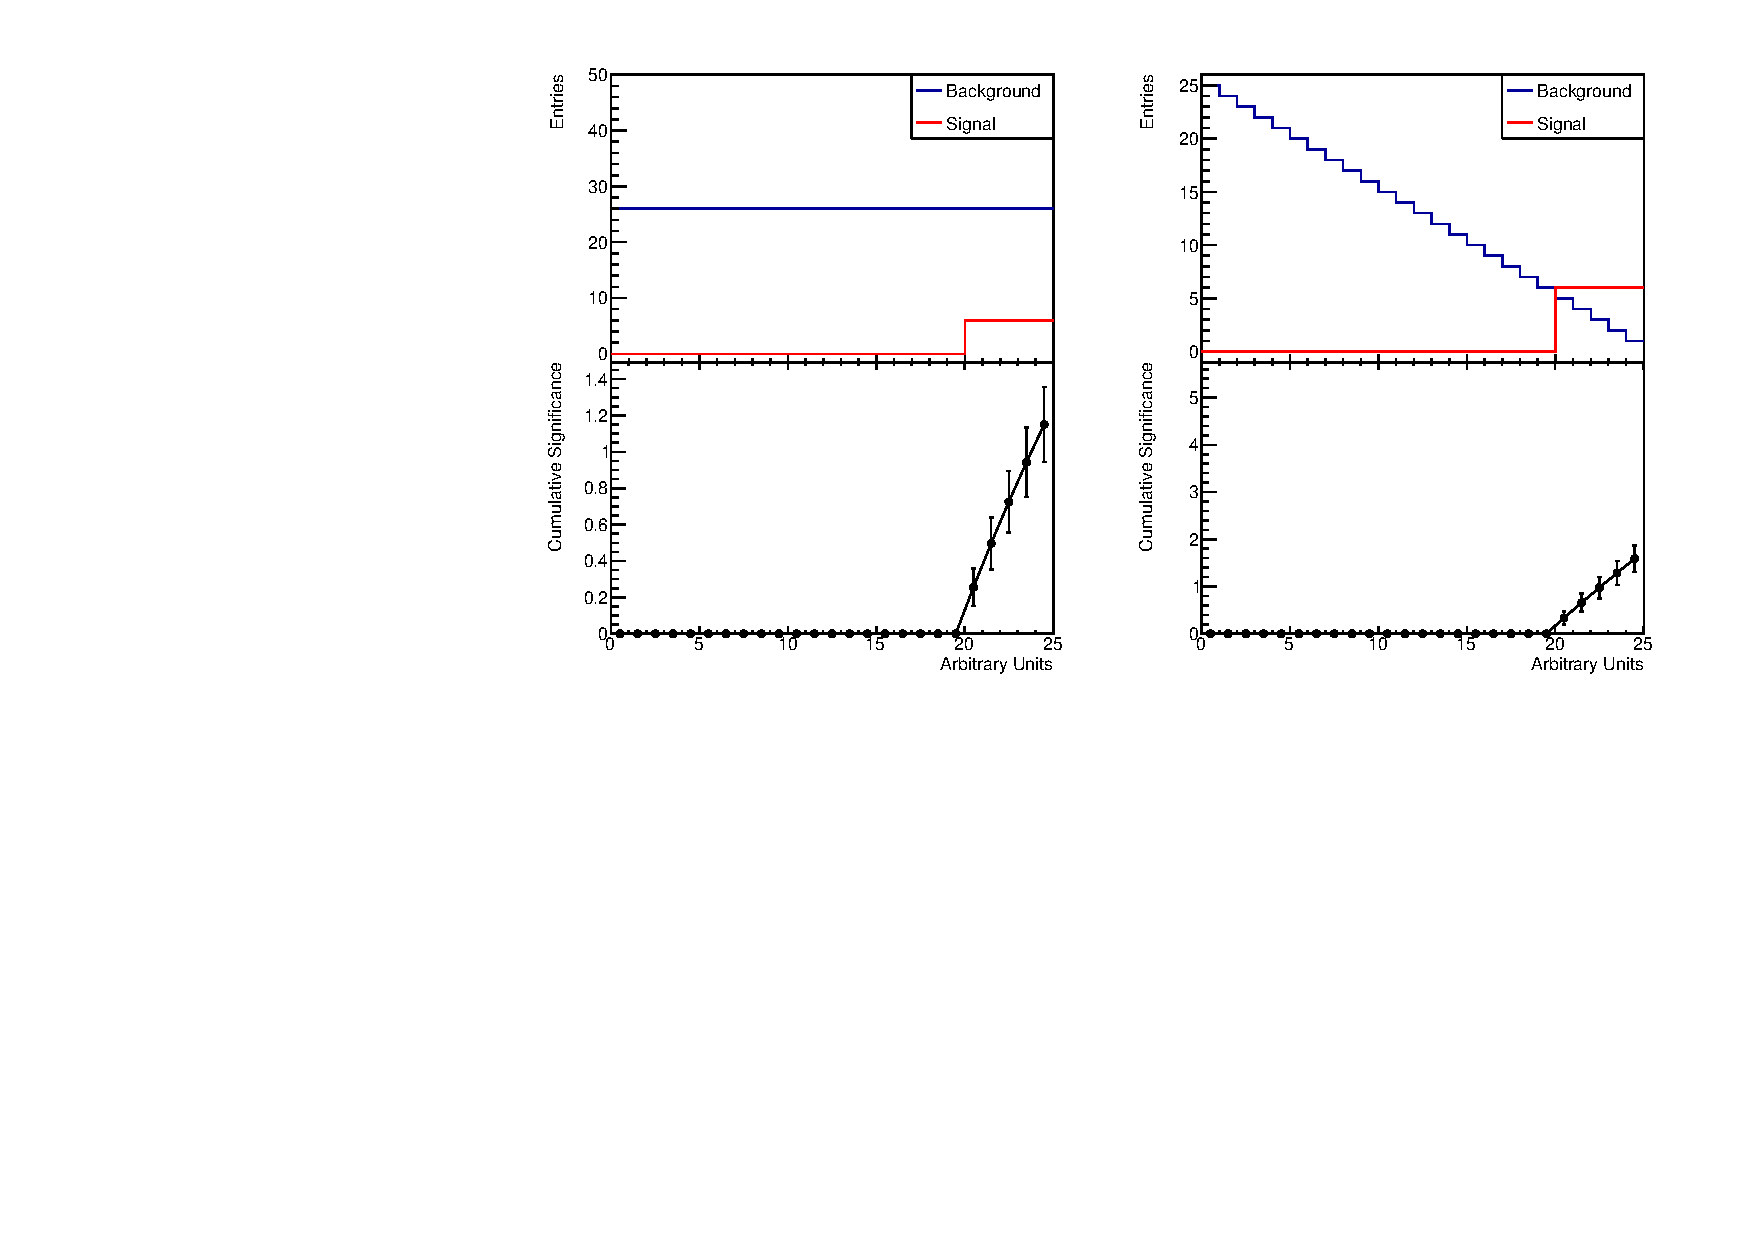
\includegraphics[width=1.\textwidth]{images/chapter7/test_cum_sig_rev.pdf}
\caption{Two distinct artificial experimental setups, with the corresponding cumulative significances plotted below. Note the rapid increase near $x=20$, indicating the optimal cut location.}
\label{test_cum_sig_rev}
}\end{figure}
\subsection{Determining the Optimal Isolation Selection Criteria}
\label{comparisons}
The cumulative significance can be used to optimise experimental analysis cuts. As was mentioned in section \ref{intro_to_flb}, isolation can be used to aid in the suppression of the \emph{fake lepton background}. The isolation selection tool used by ATLAS (see sub-section \ref{AIST}), provides two distinct classes of working points: fixed cuts and targeted efficiencies.

 In order to determine the optimal isolation selection requirement for the lepton candidates in same-sign W-boson scattering, the cumulative significances for the \textbf{topoetcone}, \textbf{fractional topoetcone}, \textbf{ptvarcone}, and \textbf{fractional ptvarcone} isolation variables were plotted. The variables prefixed by ``\textbf{fractional}'' are obtained by dividing the corresponding isolation variable of the physics object in question by its transverse momentum. Two sets of plots were produced. In the first set: lepton candidates were required to pass the targeted efficiency \textit{Gradient} isolation selection requirement. In the second set: the lepton candidates were not required to pass any isolation selection criteria. The aim of this study was to determine whether the optimal isolation requirement is: a fixed cut, \textit{Gradient}, or some composite cut combining elements of both. Given that these are plots of the cumulative significance, the value at a given point on the $x$-axis corresponds to the total significance of the events that would be gathered if a fixed cut was implemented at that point. For example, the cumulative significance of the $ee$-channel, \textbf{ptvarcone30}, no isolation selection requirement plot at the point $x = 1.0$ GeV, represents the total significance of all events included for analysis if a fixed-cut $\mathbf{ptvarcone30} < 1.0$ GeV was implemented. The same is true for the \textit{Gradient} isolation selection requirement plots, except that in this case considering the cumulative significance at some point corresponds to implementing a composite cut using both \textit{Gradient} isolation selection and a fixed-cut at the point in question. Regions where the no isolation selection requirement plots' cumulative significance is greater than the \textit{Gradient} isolation selection requirement plots' cumulative significance would suggest that a fixed-cut may perform better than \textit{Gradient} in this region. If a \textit{Gradient} isolation selection requirement plot achieves a maximum cumulative significance at a point other than that corresponding to the terminating bin, then this suggests cutting at this point to maximise the total significance of all events included for analysis.

In order to directly compare the two sets of plots, the cumulative significances for each variable in both sets were plotted together on the same set of axes, with the $ee$, $e\mu + \mu e$ , and $\mu\mu$ channels considered separately.  Only these plots produced for the direct comparison of the two sets are provided in this sub-section. For the individual plots of the cumulative significance, please see appendix \ref{appendix2}. Additionally, only the \textbf{cone30} isolation plots will be considered here, as this was the cone size used to set cuts on the variables in the Run 1 analysis. The \textbf{cone20} and \textbf{cone40} plots, for comparing the two different isolation selection requirements, display qualitatively the same behaviour as those examined here, and they are available in appendix \ref{appendix3}.

In the order of leading and sub-leading lepton respectively, figures: \ref{leading_topoetcone}, \ref{subleading_topoetcone} display the plots for the \textbf{topoetcone30} variable; figures: \ref{leading_frac-topoetcone} and \ref{subleading_frac-topoetcone} show the plots for \textbf{fractional topoetcone30} variable; figures: \ref{leading_ptvarcone}, \ref{subleading_ptvarcone} display the plots for the \textbf{ptvarcone30} variable; figures: \ref{leading_frac-ptvarcone} and \ref{subleading_frac-ptvarcone} show the plots for \textbf{fractional ptvarcone30} variable.

In general the lines for the channels, from the sub-leading lepton plots, with no isolation selection requirement, have a decrease in the cumulative significance in the terminating bin. The cumulative significances of the \textbf{topoetcone30} and \textbf{fractional topoetcone30} variables increase substantially from their starting values. This is in contrast to the \textbf{ptvarcone30} and \textbf{fractional ptvarcone30} plots, where there is very little variation in the cumulative significance except for the sub-leading lepton plots with the no isolation selection, where there is a noticeable dip in the terminating bin. These dips are due to the inclusion of overflow (mostly background) events in the final bins. The \textbf{topoetcone30} and \textbf{fractional topoetcone30} lines tend to have the channels from both the \textit{Gradient} selection and no isolation selection plots, display similar behaviour for low values of the variable but then subsequently diverge and become noticeably distinct with no overlap of the error bars.

Notice that at no point or $x$-range for any variable, channel, or leading or sub-leading lepton plot; do the solid lines corresponding to no isolation requirement, perform better than the dashed lines corresponding to the \textit{Gradient} isolation requirement. Note that the \textit{Gradient} isolation selection requirement is more effective for the $e\mu + \mu e$ and $\mu\mu$ channels where the difference between the two selections in very noticeable in all variables. In contrast, the effects on the plots in the $ee$-channel are very modest, with the errors bars overlapping, indicating that the effects are not statistically significant. This indicates that the \textit{Gradient} isolation selection requirement alone consistently performs better across all channels than any lone fixed-cut could. Although the effect is modest in the $ee$-channel.

The plots can be further interrogated to see if the cumulative significance of the dashed \textit{Gradient} isolation selection requirement lines, achieve maxima at points on the $x$-axis other than the terminating bin. This would indicate the a composite cut of using both the \textit{Gradient} isolation selection requirement with an additional fixed cut would be optimal. The $e\mu + \mu e$-channel line in figure \ref{leading_topoetcone}, the cumulative significance is seen to decrease in value in the terminating bin, so not all the \textit{Gradient} isolation selection requirement lines monotonically increase. Other lines, such as the $ee$-channel line in the same figure, show the cumulative significance achieving its maximum value at some intermediate point, in this case at $x \approx 3$. In all such cases however, the value of the cumulative significance in the terminating bin and at the maximum have overlapping errors bars. This indicates that the earlier maxima are not statically distinct from the values in the terminating bins. Hence, an additional fixed cut at these points would have a statistically negligible effect. Hence, the studies conclude that the optimal isolation requirement for lepton candidates is the \textit{Gradient} isolation requirement alone across all three channels, without any additional fixed cuts.
\begin{figure}
\centering
\begin{subfigure}{.85\textwidth}
  \centering
  \includegraphics[width=1.\linewidth]{../Desktop/workspace/l0-cone30/topoetcone30.pdf}
  \caption{}
  \label{leading_topoetcone}
\end{subfigure}
\begin{subfigure}{.85\textwidth}
  \centering
  \includegraphics[width=1.\linewidth]{../Desktop/workspace/l1-cone30/topoetcone30.pdf}
  \caption{}
  \label{subleading_topoetcone}
\end{subfigure}
\caption{Comparison of the \textbf{topoetcone30}-obtained cumulative significances for the leading (a) and sub-leading (b) lepton candidates; obtained for the case of requiring the leptons to pass the \textit{Gradient} isolation selection requirement (dashed lines) and for the case where the leptons are not required to pass any isolation selection requirement (solid lines).}
\label{comp_topoetcone}
\end{figure}
\begin{figure}
\centering
\begin{subfigure}{.85\textwidth}
  \centering
  \includegraphics[width=1.\linewidth]{../Desktop/workspace/l0-cone30/frac-topoetcone30.pdf}
  \caption{}
  \label{leading_frac-topoetcone}
\end{subfigure}
\begin{subfigure}{.85\textwidth}
  \centering
  \includegraphics[width=1.\linewidth]{../Desktop/workspace/l1-cone30/frac-topoetcone30.pdf}
  \caption{}
  \label{subleading_frac-topoetcone}
\end{subfigure}
\caption{Comparison of the \textbf{fractional-topoetcone30}-obtained cumulative significances for the leading (a) and sub-leading (b) lepton candidates; obtained for the case of requiring the leptons to pass the \textit{Gradient} isolation selection requirement (dashed lines) and for the case where the leptons are not required to pass any isolation selection requirement (solid lines).}
\label{comp_frac-topoetcone}
\end{figure}
\begin{figure}
\centering
\begin{subfigure}{.85\textwidth}
  \centering
  \includegraphics[width=1.\linewidth]{../Desktop/workspace/l0-cone30/ptvarcone30.pdf}
  \caption{}
  \label{leading_ptvarcone}
\end{subfigure}
\begin{subfigure}{.85\textwidth}
  \centering
  \includegraphics[width=1.\linewidth]{../Desktop/workspace/l1-cone30/ptvarcone30.pdf}
  \caption{}
  \label{subleading_ptvarcone}
\end{subfigure}
\caption{Comparison of the \textbf{ptvarcone30}-obtained cumulative significances for the leading (a) and sub-leading (b) lepton candidates; obtained for the case of requiring the leptons to pass the \textit{Gradient} isolation selection requirement (dashed lines) and for the case where the leptons are not required to pass any isolation selection requirement (solid lines).}
\label{comp_ptvarcone}
\end{figure}
\begin{figure}
\centering
\begin{subfigure}{.85\textwidth}
  \centering
  \includegraphics[width=1.\linewidth]{../Desktop/workspace/l0-cone30/frac-ptvarcone30.pdf}
  \caption{}
  \label{leading_frac-ptvarcone}
\end{subfigure}
\begin{subfigure}{.85\textwidth}
  \centering
  \includegraphics[width=1.\linewidth]{../Desktop/workspace/l1-cone30/frac-ptvarcone30.pdf}
  \caption{}
  \label{subleading_frac-ptvarcone}
\end{subfigure}
\caption{Comparison of the \textbf{fractional-ptvarcone30}-obtained cumulative significances for the leading (a) and sub-leading (b) lepton candidates; obtained for the case of requiring the leptons to pass the \textit{Gradient} isolation selection requirement (dashed lines) and for the case where the leptons are not required to pass any isolation selection requirement (solid lines).}
\label{comp_frac-ptvarcone}
\end{figure}
\section{Using the Cumulative Significance to Optimise Other Analysis Cuts}
The cumulative significance approach to analysis cut optimisation, described in sub-section \ref{description_of_cum_sig} and used in sub-section \ref{comparisons}, can also be used to optimise cuts on other variables. In this sub-section the cumulative significance approach is applied to three variables: the lepton invariant mass ($m_{\ell \ell}$), the jet invariant mass ($m_{jj}$), and the jet separation rapidity ($\Delta y_{jj}$). In each case the histogram and corresponding significance are plotted for the variable immediately before its associated cut is implemented. See section \ref{event_selection} for the ordered list of analysis cuts.

Figures \ref{ee_mll}, \ref{emme_mll}, and \ref{mm_mll} show the lepton invariant mass plots for the $ee$, $e\mu + \mu e$, and $\mu\mu$ channels respectively. While the $e \mu +\mu e$ plot suggests not implementing a cut at all\footnote{This is not in agreement with the current (as of writing) same-sign W-boson scattering analysis cut of: $m_{\ell \ell} > 20$ GeV, across all channels.}, both the $ee$ and $\mu\mu$ suggests cutting out the region $55 < m_{\ell \ell} < 95$ GeV. However, since the dominant background contributions are $Z$ + $jets$ events, and the mass spectrum peaks at the Z-mass of approximately 90 GeV, this can be interpreted as an argument to implement a Z-mass veto. This is done in a subsequent cut as listed in section \ref{event_selection} cut 5. which vetoes events failing: $76.2 < m_{ee} < 106.2$ GeV, only in the $ee$ channel.\footnote{Note that this mass region, cut out by the Z-mass veto, does not have the same bounds as the cut suggested by the looking at the cumulative significance. This is because the cumulative significance will dip and rise asymmetrically about the Z-mass peak at 91.2 GeV, in response to the sudden increases and then subsequent decreases in the number of background events.} This indicates that a Z-mass veto should also be imposed on $\mu\mu$-channel events.

Figures \ref{ee_mjj}, \ref{emme_mjj}, and \ref{mm_mjj} show the jet invariant mass plots for the $ee$, $e\mu + \mu e$, and $\mu\mu$ channels respectively; while figures \ref{ee_DYjj}, \ref{emme_DYjj}, \ref{mm_DYjj} show the jet separation rapidity plots in the same channel order. Note that the cumulative significances for both of these variables and for all channels suggest not implementing any associated cut. This is in opposition to current same-sign W-boson scattering analysis cuts on these variables of $m_{jj} > 500$ GeV and $\Delta y_{jj} > 2.4$.

\begin{figure}
	\centering
		\includegraphics[width = 0.5\textwidth]{../results/gamma/70_Grad_mc_only-ee/plots/ee-CutTriggerMatch-Mll-log.png}
		\caption{Histogram of the lepton invariant mass ($ee$ channel). The corresponding cumulative significance curve is plotted below.}
		\label{ee_mll}
\end{figure}
\begin{figure}
	\centering
		\includegraphics[width = 0.5\textwidth]{../results/gamma/70_Grad_mc_only-emme/plots/emme-CutTriggerMatch-Mll-log.png}
		\caption{Histogram of the lepton invariant mass ($e \mu + \mu e$ channel). The corresponding cumulative significance curve is plotted below.}
		\label{emme_mll}
\end{figure}
\begin{figure}
	\centering
		\includegraphics[width = 0.5\textwidth]{../results/gamma/70_Grad_mc_only-mm/plots/mm-CutTriggerMatch-Mll-log.png}
		\caption{Histogram of the lepton invariant mass ($\mu\mu$ channel). The corresponding cumulative significance curve is plotted below.}
		\label{mm_mll}
\end{figure}

\begin{figure}
	\centering
		\includegraphics[width = 0.5\textwidth]{../results/gamma/70_Grad_mc_only-ee/plots/ee-Cut2JSSBVeto-Mjj-lin.png}
		\caption{Histogram of the jet invariant mass ($ee$ channel). The corresponding cumulative significance curve is plotted below.}
		\label{ee_mjj}
\end{figure}
\begin{figure}
	\centering
		\includegraphics[width = 0.5\textwidth]{../results/gamma/70_Grad_mc_only-emme/plots/emme-Cut2JSSBVeto-Mjj-lin.png}
		\caption{Histogram of the jet invariant mass ($e \mu + \mu e$ channel). The corresponding cumulative significance curve is plotted below.}
		\label{emme_mjj}
\end{figure}
\begin{figure}
	\centering
		\includegraphics[width = 0.5\textwidth]{../results/gamma/70_Grad_mc_only-mm/plots/mm-Cut2JSSBVeto-Mjj-lin.png}
		\caption{Histogram of the jet invariant mass ($\mu\mu$ channel). The corresponding cumulative significance curve is plotted below.}
		\label{mm_mjj}
\end{figure}

\begin{figure}
	\centering
		\includegraphics[width = 0.5\textwidth]{../results/gamma/70_Grad_mc_only-ee/plots/ee-Cut2JSSMjj-DYjj-lin.png}
		\caption{Histogram of the jet separation rapidity ($ee$ channel). The corresponding cumulative significance curve is plotted below.}
		\label{ee_DYjj}
\end{figure}
\begin{figure}
	\centering
		\includegraphics[width = 0.5\textwidth]{../results/gamma/70_Grad_mc_only-emme/plots/emme-Cut2JSSMjj-DYjj-lin.png}
		\caption{Histogram of the jet separation rapidity ($e \mu + \mu e$ channel). The corresponding cumulative significance curve is plotted below.}
		\label{emme_DYjj}
\end{figure}
\begin{figure}
	\centering
		\includegraphics[width = 0.5\textwidth]{../results/gamma/70_Grad_mc_only-mm/plots/mm-Cut2JSSMjj-DYjj-lin.png}
		\caption{Histogram of the jet separation rapidity ($\mu\mu$ channel). The corresponding cumulative significance curve is plotted below.}
		\label{mm_DYjj}
\end{figure}
